\section{Independence of the axioms}\label{sec:necessity}

For each of the axioms \axN, \axCM, \axLI, \axRC{} and \axRM{} we give a loss ratio that satisfies the
remaining axioms and is not of the form in Theorem~\ref{thm:A} or~\ref{thm:B}. Axiom \axP{} defines the implied
premium, through which the other axioms are formulated, and is therefore not treated in the same way; see
Remark~\ref{rem:labels} for what is lost without it. Table~\ref{tab:witnesses} summarizes the examples.

\begin{table}[ht]
\centering\small
\begin{tabularx}{\textwidth}{@{}l>{\raggedright\arraybackslash}p{4.6cm}>{\raggedright\arraybackslash}X@{}}
\toprule
\textbf{Dropped} & \textbf{Witness} & \textbf{Why it is a witness}\\
\midrule
\axN & $\bracket{I_h}{\kappa I_g}$, $\kappa>0$, $\kappa\ne1$
 & All other axioms hold; $\LR(c)=1/\kappa\ne1$.\\
\axCM & $\bracket{\max(I_{\sqrt t},I_{\min(1,1.5t)})}{\E}$
 & Implied risk measure is cash additive but not comonotonic additive.\\
\axLI & $\bracket{\E_Q}{\E}$, $Q\ne P$ with bounded density
 & All other axioms hold; $\E_Q$ is not law invariant.\\
\axRC{} (Thm.~\ref{thm:A}) & $\bracket{I_h}{\E}$ with $h$ continuous, not of bounded variation
 & Uniform continuity fails; $h$ is not of bounded variation.\\
\axRM{} (Thm.~\ref{thm:B}) & $\bracket{I_h}{\E}$, $h(t)=t+\tfrac14\sin2\pi t$
 & $h$ is not monotone, so no distortion pair represents it.\\
\bottomrule
\end{tabularx}
\caption{Witnesses for the axioms of Theorems~\ref{thm:A} and~\ref{thm:B}.}\label{tab:witnesses}
\end{table}

\begin{example}[Independence of \axN: a loading on sure losses]
Fix $\kappa>0$, $\kappa\neq1$, and let $\LR=\bracket{I_h}{\kappa I_g}$ with distortions $h,g$. The cash line of
$X$ is $(I_h(X)+c)/(\kappa(I_g(X)+c))$, non-finite only at $c=-I_g(X)$, so \axP{} holds with $\Pi=I_g$. With these
weights the pooling identity holds because $I_h$ and $I_g$ are comonotonic additive; \axLI{} holds, and so do
\axRM{} and \axRC, since $\Pi=I_g$ and $\rho_D=\Pi\cdot\LR=I_h/\kappa$ are monotone and Lipschitz. But $\LR(c)=1/\kappa\ne1$, whereas every ratio in Theorem~\ref{thm:A} has value $1$ at sure losses. So the
normalization is not harmless: it is what excludes loadings on sure losses. (We conjecture, but have not proved,
that an analogue of Theorem~\ref{thm:A} with a known loading $\kappa$ holds with $\LR=\bracket{I_h}{\kappa I_g}$.)
\end{example}

\begin{example}[Ordinal information is not enough]\label{ex:cube}
Let $h\ne g$ be distortions and $\LR'=\psi\circ\bracket{I_h}{I_g}$ with $\psi(t)=t^3$ and $\psi$ fixing the
non-finite values. Since $\psi$ maps $\R$ to $\R$, $\LR'$ has the same price points as $\bracket{I_h}{I_g}$, so
\axP{} holds with $\Pi=I_g$; \axN{} holds because $1^3=1$; \axLI{} holds, and so does the mediant inequality,
because $\psi$ is increasing. But $\LR'$ is not of the form in Theorem~\ref{thm:A}: at a book $X$ with
$I_h(X)\neq I_g(X)$ (for instance an indicator at a point where $h\ne g$), the cash line
$\big((I_h(X)+c)/(I_g(X)+c)\big)^3$ has a pole of order three, while every cash line in Theorem~\ref{thm:A} has a
simple pole. Hence \axCM{} fails. (This example is an illustration, not a witness in the strict sense: on
$D$, $\Pi\cdot\LR'=I_h^3/I_g^2$ is neither uniformly continuous nor monotone.) Betweenness-type, ordinal information determines the loss ratio only up to an
increasing transformation, as for \citet{chew1983} and \citet{dekel1986}; the cardinal axiom \axCM{} cannot be
avoided.
\end{example}

\begin{example}[Independence of \axCM]
Let $\LR=\bracket{\rho}{\E}$ with $\rho=\max(I_{\sqrt t},I_{\min(1,1.5t)})$. \axP{} holds with $\Pi=\E$, \axN{}
holds, and the implied risk measure is $\rho$, a maximum of cash-additive maps; \axLI, \axRM{} and \axRC{} hold. Take
$E\subset B$ with $P(B)=0.5$, $P(E)=0.1$ and $X=\1_B+\1_E$. Then $\rho(\1_B)=\max(0.707,0.75)=0.75$ and
$\rho(\1_E)=\max(0.316,0.15)=0.316$, with sum $1.066$, while $\rho(X)=\max(0.707+0.316,\ 0.75+0.15)=1.023$. So $\rho$
is not comonotonic additive and \axCM{} fails by Lemma~\ref{lem:comon}(a).
\end{example}

\begin{example}[Independence of \axLI]
Let $Z=dQ/dP$ be bounded, non-constant, $Z\ge0$ and $\E Z=1$, and $\LR=\bracket{\E_Q}{\E}$. \axP{} holds with
$\Pi=\E$, \axN{} holds, \axCM{} holds by Lemma~\ref{lem:comon}(b) because $\E_Q$ and $\E$ are additive, and \axRM,
\axRC{} hold. But $\E_Q(\1_A)=Q(A)$ is not a function of $P(A)$, so the implied risk measure is not of the form
$I_h$. Without \axLI{} the class is exactly that of Theorem~\ref{thm:A0}.
\end{example}

\begin{example}[Independence of \axRC{} in Theorem~\ref{thm:A}]
Let $h(t)=t\big(1+\tfrac12\sin(1/t)\big)/\big(1+\tfrac12\sin1\big)$, continuous with $h(0)=0$, $h(1)=1$, and not of
bounded variation (Figure~\ref{fig:witness}) ($\int|h'|$ diverges at $0$). Let $\LR=\bracket{I_h}{\E}$. \axP, \axN{} and \axLI{} are clear;
$I_h$ is norm continuous (survival functions converge off a countable set, and dominated convergence applies)
and additive on simple comonotone positions by the layer computation, hence comonotonic additive, so \axCM{}
holds. The implied risk measure is $I_h$, and by Lemma~\ref{lem:bv} \axRC{} would force $h$ to be of bounded
variation. So \axRC{} fails and no pair in $\Hset_1^2$ represents $\LR$.
\end{example}

\begin{remark}[Some regularity is indispensable]
\axP, \axN, \axCM{} and \axLI{} alone do not force continuity. Using a Hamel basis one obtains
$\rho=\E+\varphi\circ I_k$ with $k(t)=t(1-t)$ (so that $I_k$ vanishes on constants and is cash invariant) and
$\varphi$ additive but discontinuous. Then $\bracket{\rho}{\E}$ satisfies \axP, \axN, \axCM{} and \axLI{} and is not of
the form in Theorem~\ref{thm:A}. This witness uses the axiom of choice; all the others are constructive.
\end{remark}

\begin{example}[Independence of \axRM{} in Theorem~\ref{thm:B}]
Let $h(t)=t+\tfrac14\sin2\pi t\in\Hset_1$ (Figure~\ref{fig:witness}), so $h(0.4)\approx0.547>h(0.6)\approx0.453$, and
$\LR=\bracket{I_h}{\E}$. All other axioms hold (\axRC{} by the Lipschitz bound), but the implied risk measure
$I_h$ is not monotone, and no distortion pair represents $\LR$ because the pair is unique.
\end{example}

\begin{figure}[ht]
\centering
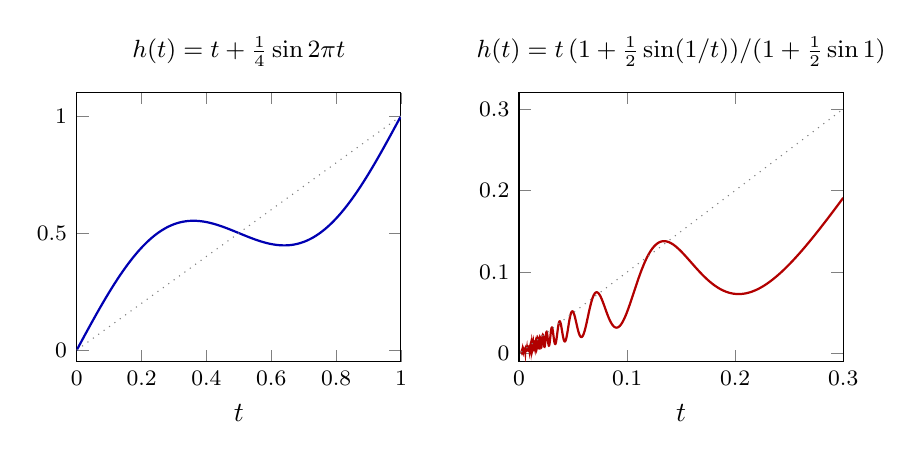
\begin{tikzpicture}
\begin{axis}[name=l,width=0.47\textwidth,height=5cm,xmin=0,xmax=1,ymin=-0.05,ymax=1.1,xlabel={$t$},
  title={\small $h(t)=t+\frac14\sin2\pi t$},tick label style={font=\footnotesize},samples=200,domain=0:1]
\addplot[thick,blue!70!black] {x+0.25*sin(deg(2*pi*x))};
\addplot[gray,dotted] {x};
\end{axis}
\begin{axis}[at={(l.south east)},xshift=1.5cm,width=0.47\textwidth,height=5cm,xmin=0,xmax=0.3,ymin=-0.01,ymax=0.32,
  xlabel={$t$},title={\small $h(t)=t\,(1+\frac12\sin(1/t))/(1+\frac12\sin1)$},tick label style={font=\footnotesize},
  samples=2000,domain=0.002:0.3]
\addplot[thick,red!70!black] {x*(1+0.5*sin(deg(1/x)))/(1+0.5*sin(deg(1)))};
\addplot[gray,dotted] {x};
\end{axis}
\end{tikzpicture}
\caption{Numerator distortions of the witnesses for \axRM{} (left: of bounded variation, not monotone) and for
\axRC{} (right, near $0$: continuous, not of bounded variation). The dotted line is the identity.}\label{fig:witness}
\end{figure}

\subsection{Witnesses for the actuarial axioms}

\begin{table}[ht]
\centering\small
\begin{tabularx}{\textwidth}{@{}l>{\raggedright\arraybackslash}p{4.6cm}>{\raggedright\arraybackslash}X@{}}
\toprule
\textbf{Dropped} & \textbf{Witness on $\Xp$} & \textbf{Reason}\\
\midrule
(A2) & $\E_Q/\E$ & $N_0$ lies in a closed hyperplane, so (A0) holds; not law invariant.\\
(A3) & $C_h/\E$, $h=t+\tfrac14\sin2\pi t$ & $\rho(\1_A)>\rho(\1_B)$ for $\1_A\le\1_B$, $P(A)=0.4,P(B)=0.6$.\\
(A3$_s$) & $C_h/\E$, $h$ continuous non-BV & Extensions exist; $h$ is not of bounded variation.\\
(A4a) & $\E/\max(C_{\sqrt t},C_{\min(1,1.5t)})$ & Premium is not comonotonic additive (numbers above); (A4b) holds.\\
(A4b) & $\max(C_{\sqrt t},C_{\min(1,1.5t)})/\E$ & $\bar\Pi=\E$ additive, but $\bar\Pi\LR_0$ is not.\\
(A5) & $C_h/C_g$ with $g=(2t-1)^+$, $h=g^2$, and $\LR_0:=1$ where $C_g=0$ & $\LR_0$ jumps: $\LR_0(\1_B+n^{-1}\1_C)=\tfrac12$ while $\LR_0(\1_B)=1$ for $P(B)\le\tfrac12$, $C\supset B$, $P(C)=\tfrac34$.\\
\bottomrule
\end{tabularx}
\caption{Witnesses for (A2)--(A5) on the actuarial domain. In each case all other axioms hold.}\label{ex:A5}
\end{table}

Axioms (A0) and (A1) define $\rho$ and $\Pi$ on $\Xp\setminus N_0$, through which the remaining axioms are stated, so they
are not treated as independent axioms. Two examples illustrate the identification they provide. If $\LR_0\equiv1$,
(A0) fails and $(\mathrm{id},\mathrm{id})$ and $(\sqrt\cdot,\sqrt\cdot)$ both represent $\LR_0$. If $\LR_0=(C_h/C_g)^3$ with
distortions $h\ne g$ and $g>0$, then $N_0$ is that of $C_h/C_g$, but (A1) fails, because the cash line has a pole of
order three at $-C_g(X)$ for $X\notin N_0$.

\begin{remark}[Atomlessness]
Atomlessness is used to attain every $p\in[0,1]$ as $P(A)$. On a space with atoms, $(h,g)$ is identified only
on the range of $P$.
\end{remark}
